\subsection{Simulationserweiterung}
\subsubsection{Steuerung}
\label{sec_waypoint}
Wie im Kapitel \ref{sec_auvSimGrundlage} Grundlagen beschrieben, wird in der bestehenden Simulation ein \texttt{\gls{lanefollow}}, der eine Linie zwischen einem \textit{old\_waypoint} und einem \textit{new\_waypoint} bildet, verwendet.
Die Schnittstelle zur Steuerung bildet somit die Kombination aus den beiden Wegpunkten. Die Berechnung der Wegpunkte wird auf Basis des Polynoms aus dem Schätzverfahren generiert.\\
Zunächst wird die Position des \gls{auv}s durch die aktuelle Transformationsmatrix in das alternative Weltkoordinatensystem (siehe Absatz \ref{alterWorldCoords}) transformiert. Es wird der der transformierten Position des \gls{auv}s nächstgelegene Punkt auf dem Polynom zur  berechnet. Dieser Punkt dient als Zentrum für einen Kreis zur Bestimmung der Wegpunkte. Mithilfe der Kreisgleichung [Gleichung \ref{circEq}] werden die zwei Schnittpunkte des Polynoms mit dem Kreis berechnet. Da durch die Transformationsmatrix sichergestellt wird, dass das \gls{auv} in Richtung der $X-Achse$ fährt, kann problemlos der Schnittpunkt mit höherem $x$-Wert als \textit{next\_waypoint} und dementsprechend der zweite als \textit{old\_waypoint} verwendet werden. Es wird davon ausgegangen, dass bei einem solch kleinen Kreisradius (zwischen 5 und 10 Metern) nicht mehr als zwei Schnittpunkte zwischen Polynom und Kreis vorhanden sind. Sollte dies der Fall sein, wäre das Polynom viel zu stark gekrümmt, um noch verfolgt zu werden. Im Szenario dieser Arbeit gibt es auch keine Objekte, die eine solch starke Krümmung aufweisen.\\
Der letzte Schritt besteht aus der \gls{transform} der Wegpunkte in das reale VRML-Koordinatensystem mithilfe der inversen Transformationsmatrix.
Das Verfahren ist in Abbildung \ref{wpCircle} grafisch dargestellt.

\begin{ownequation}[H]
\begin{equation}
0 = (X_{test}-Center_X)^2+(Y_{test}-Center_Y)^2 - r^2
\end{equation}
\caption[Kreisgleichung zum Test, ob ein Punkt auf einem Kreis liegt.]{Kreisgleichung zum Test ob ein Punkt $X_{test},Y_{test}$ auf einem Kreis liegt. $Center_X$ und $Center_Y$ bilden hierbei den Mittelpunkt eines Kreises mit Durchmesser $r$.}
\label{circEq}
\end{ownequation}

\begin{figure}[H]
\centering
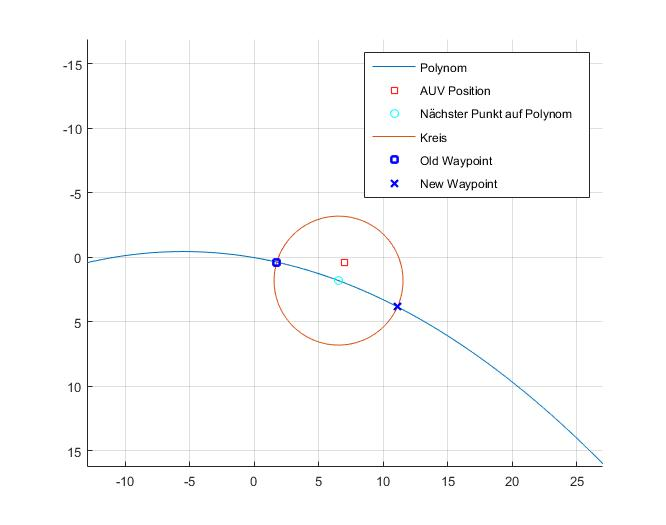
\includegraphics[scale=0.8]{waypointProvier.jpg}
\caption[Verfahren zur Bestimmung der Wegpunkte]{Verfahren zur Bestimmung der Wegpunkte. Der Wegpunkt wird im alternativen Weltkoordinatensystem bestimmt. Hierbei wird ein Kreis um den nächsten Punkt vom \gls{auv} auf dem Polygon bestimmt. Die Schnittpunkte des Kreises bilden die Wegpunkte für die \gls{auv}-Steuerung.}
\label{wpCircle}
\end{figure}
\subsubsection{Kamerabilder}
Da die Simulation in der ursprünglichen Form noch sehr \textit{klinische} Bilder generierte, mussten diese Bilder künstlich verschlechtert und die Sichtverhältnisse eingeschränkt werden, um realistische Eingangsbilder zu erzeugen. In Abbildung \ref{simPics} ist von links nach rechts ein ursprüngliches Kamerabild, ein verschlechtertes Bild und ein sehr stark verschlechtertes Bild zu sehen. Die Testläufe der Arbeit wurden mit dem Verschlechterungsgrad des mittleren Bildes durchgeführt. Die Objekterkennung wurde zudem noch mit Bildern, wie dem rechten Bild getestet.
\begin{figure}[H]
\begin{tabular}{ccc}
\subfloat[Ursprüngliches Bild]{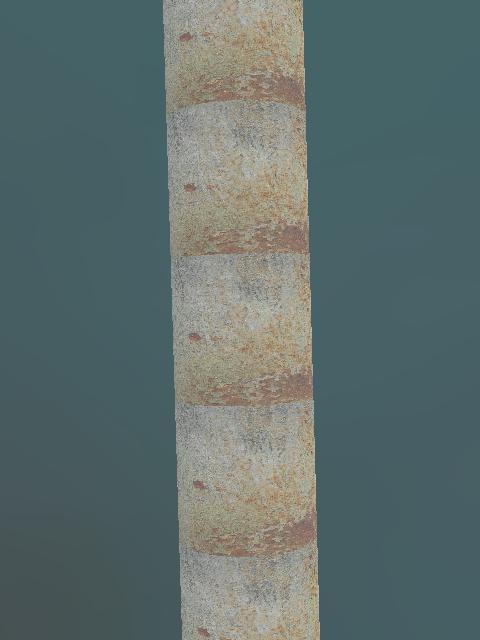
\includegraphics[scale=0.8,width=0.33\textwidth]{/imageProcessing/gradeOptimal.jpg}}&
\subfloat[Bild verschlechtert mit leichter \gls{blur} und geringem Pixelrauschen]{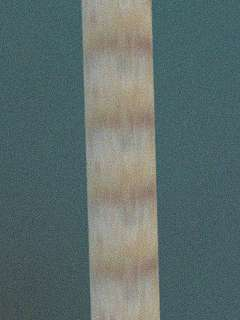
\includegraphics[scale=0.8,width=0.33\textwidth]{/imageProcessing/graeOk.jpg}}&
\subfloat[Sichtverhältnisse verschlechtert mit \gls{blur} und geringem Pixelrauschen]{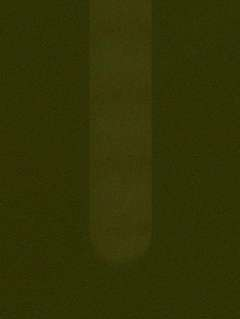
\includegraphics[scale=0.8,width=0.33\textwidth]{/imageProcessing/Prinzip/sim2,5Vis.jpg}}\\
\subfloat[Sichtverhältnisse stark verschlechtert mit \gls{blur} und geringem Pixelrauschen]{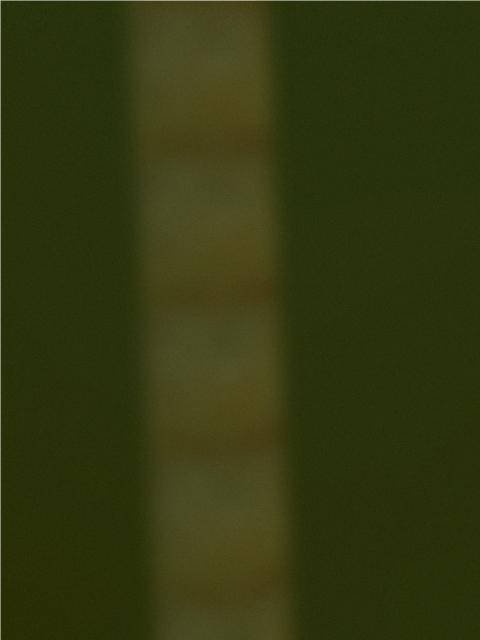
\includegraphics[scale=0.8,width=0.33\textwidth]{/imageProcessing/gradeTestQuali.jpg}}&
\subfloat[Sichtverhältnisse sehr stark verschlechtert, simulierte Reflexion des Wassers mit \gls{blur} und geringem Pixelrauschen]{
\includegraphics[scale=0.8,width=0.33\textwidth]{/imageProcessing/gradeschlecht.jpg}}\label{img_badSeight}&
\end{tabular}
\caption[Simulationsbilder]{Simulationsbilder. \textit{a)} zeigt das ursprüngliche Bild. In \textit{b)} bis \textit{e)} wird das Bild auf verschiedenen Arten verschlechtert. Die meisten Testläufe wurden mit der Verschlechterung von \textit{b)} und \textit{d)} durchgeführt. Tests unter sehr schlechten Bedingungen mit einem Grad der Verschlechterung aus \textit{e)}}
\label{simPics}
\end{figure}